\section{Discrimination}
\label{sec:Single-cell decoding}
\begin{exm}
  \label{exm:mokey experiment}
  In the experiments performed by Britten et al. (1992).,
a monkey was trained to discriminate between two directions of motion
of a visual stimulus which was a pattern of dots on a video monitor. The percentage of dots that move together in the fixed direction is
called the coherence level. By varying the degree of coherence shown by
pictures, the task of detecting the movement direction can be made more or less
diffcult.
\begin{center} 
 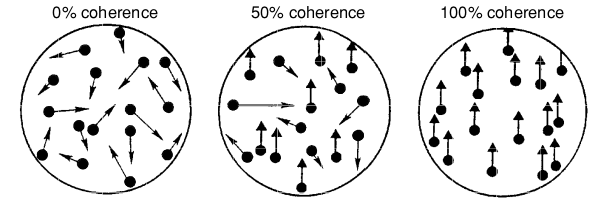
\includegraphics[scale = 0.3]{./png/3-1}
\end{center}
\end{exm}
\begin{defn}[plus and minus]
  \label{defn:plus and minus}
  The preferred direction was called \emph{plus} (\rm{or} $+$ ) 
direction that produced the maximum response
in that neuron, and  its opposite direction is called the \emph{minus}
 (\rm{or} $-$ ) direction.
\end{defn}
\begin{exm}
  \label{fig:random-dot motion-
discrimination task}
  During the same experiment in Example \ref{exm:mokey experiment}, the judgment
  accuracy of the monkey and the optic nerve coding signal activity in
  the MT area were recorded. The experimental results show that: first,
  the coding of MT neural activity is basically sufficient for judging
  the direction; second, at high coherence levels, the fring-rate distributions
corresponding to the two directions are fairly well separated, while
at low coherence levels, they merge.
\begin{center}
  \centering
 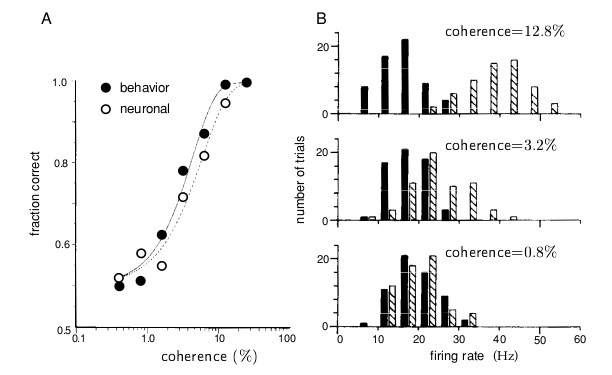
\includegraphics[scale = 0.4]{png/3-2AB}
  \label{fig:3.2A}
\end{center}

\end{exm}

\begin{rem}
  Although spike count rates take only discrete values, it is more
  convenient to treat $r$ as a continuous variable for our
  discussion. Treated as probability densities, these two
  distributions are approximately Gaussian with the same variance, $\sigma_{r}^{2}$, but different means,
$\left\langle r \right\rangle_{+}$ for the plus direction and $\left\langle r \right\rangle_{-}$ for the minus direction.
\end{rem}

\begin{defn}[discriminability]
  \label{defn:discriminability}
  A convenient
measure of the separation between the distributions is the
\emph{discriminability}
\begin{equation}
  \label{eq:3.4}
  d'=\frac{\left\langle r \right\rangle_{+}-\left\langle r \right\rangle_{-}}{\sigma_{r}}.
\end{equation}
\end{defn}


\begin{rem}
 
Decoding involves using the neural
response to determine in which of the two possible directions the
stimulus moved for Example \ref{exm:mokey experiment}. A simple decoding procedure in this case is to determine the fring rate
$r$ during a trial and compare it to a threshold number $z$. If $r
\geq z$, we report “plus”; otherwise we report “minus”.
\end{rem}

\begin{defn}[size and power]
  \label{defn:size and power}
    Below are the probabilities of answering plus for both given the conditions:
  \begin{enumerate}[(i)]
  \item The probability that it will give the answer “plus”
when the stimulus is moving in the plus direction is the conditional probability that $r\geq z$ given a plus
stimulus, $\alpha(z)=P[r\geq z|+]$, called \emph{size} or \emph{false
  alarm} rate of the test.
\item The probability that it will give the answer “plus”
when the stimulus is actually moving in the minus direction (called a false
alarm) is similarly $\beta(z)=P[r\geq z|-]$, called \emph{power} or \emph{hit} rate of the test.
\end{enumerate}

These two probabilities completely determine the performance of the decoding procedure because the probabilities for the other two cases
\begin{center}
  \begin{tabular}[h]{|c|cc|}
\hline
         & \multicolumn{2}{c|}{probablity}          \\ \hline
stimulus & \multicolumn{1}{c|}{correct} & incorrect \\ \hline
$+$        & \multicolumn{1}{c|}{$\beta$}        &$1-\beta$       \\ \hline
$-$       & \multicolumn{1}{c|}{$1-\alpha$}     & $\alpha$         \\ \hline
\end{tabular}
\end{center}
\end{defn}


\subsection{ROC Curves}
\begin{defn}
  \label{def:ROC curves}
  The \emph{receiver operating characteristic} (\textbf{ROC}) curve is
  traced out as a function of the threshold $z$. Each point on an ROC
  curve corresponds to a different value of $z$. The $x$ coordinate of
  the point is $\alpha$, the size of the test for this value of $z$
 and the $y$ coordinate is $\beta$. ROC curve provides a way of
 evaluating how test performance depends on the choice of  $z$ and
 indicates how the size and power of a test trade off as the threshold
 is varied.
\end{defn}

\begin{exm}
  \label{exm:ROC curves}
The figure shows ROC curves computed by Britten et al. for several different values of the stimulus coherence.
\begin{enumerate}[(i)]
\item At high coherence levels, when
the task is easy, the ROC curve rises rapidly from $\alpha(z)=0$,
$\beta(z)=0$ as the threshold is lowered from a high value, and the
probability $\beta(z)$ of a correct “plus” answer quickly approaches
$1$ without a concomitant increase in $\alpha(z)$. As the threshold is
lowered further, the probability of giving the answer “plus” when
the correct answer is “minus” also rises, and $\alpha(z)$ increases.
\item At lower high coherence levels, when the task is difficult, the
  curve rises more slowly as $z$ is lowered.
\item At quite low coherence levels, the task is impossible, in that
  the test merely gives random answers, the curve will lie along the diagonal $\alpha=\beta$, because the probabilities of answers being correct and incorrect are equal.
\end{enumerate}
\begin{center}
    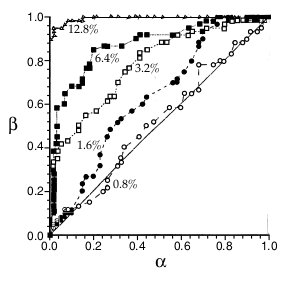
\includegraphics[scale = 0.5]{png/3-3}
 \end{center}
\end{exm}

\begin{rem}
  Examination of Example \ref{exm:ROC curves} suggests a relationship between
  the area under the ROC curve and the level of performance on the
  task. When the ROC curve in Example \ref{exm:ROC curves} lies along the diagonal, the
  area underneath it is $1/2$, which is the probability of a correct
  answer in this case (given any threshold). When the task is easy and
  the ROC curve hugs the left axis and upper limit, the area under it approaches $1$, which is again the
  probability of a correct answer (given an appropriate threshold). The
  area underneath the ROC curve is the probability of a correct answer
  in the most cases (given an appropriate threshold).

  However, the precise relationship between task performance and the area under
the ROC curve is complicated by the fact that different threshold values can be
used. This ambiguity can be removed by considering a slightly different
task, called \emph{two-alternative forced choice}.
\end{rem}

\begin{ntn}
  \label{ntn:two-alternative forced choice}
  For \emph{two-alternative forced choice}, the stimulus is presented
twice, once with motion in the plus direction and once in the minus di-
rection. The task is to decide which presentation corresponded to the plus
direction, given the fring rates on both trials, $r_1$ and $r_2$. A natural exten-
sion of the test procedure we have been discussing is to answer trial 1 if
$r_1 \geq r_2 $ and otherwise answer trial 2. This removes the threshold variable
from consideration.
\end{ntn}

\begin{prop}
  \label{prop:two-alternative correct probability}
 In the two-alternative force-choice task, the value of $r$ on one trial serves
as the threshold for the other trial. Then the probability of getting the correct answer
\begin{equation}
  \label{eq:3.6}
  P[\rm{correct}]=\int_{0}^{\infty}{p[z|-]\beta(z)dz}.
\end{equation}
 \begin{proof}
 For example, if the order of stimulus presentation is plus, then minus, the comparison procedure we have
outlined will report the correct answer if $r_1 \geq z$ where $z=r_2$,
and this has probability $P[r_1\geq z|+]=\beta(z)$ with $z=r_2$. For
small $\Delta z$, the probability that $r_2$ takes a value in the range
between $z$ and $z+\Delta z$ when the second trial has a minus
stimulus is $p[z|-]\Delta z$, where $p[z|-]$ is the conditional
fring-rate probability density for a fring rate $r=z$. Integrating over all values of $z$
gives the answer.
 \end{proof}
\end{prop}


\begin{prop}
  \label{prop:size}
The probability of getting the correct answer in the
Equation \ref{eq:3.6} can be transformed into
\begin{equation}
  \label{eq:3.5}
  P[\rm{correct}]=\int_0^1\beta d\alpha.
\end{equation}

 \begin{proof} 
   $\alpha(z)$ mentioned in definition \ref{defn:size and power}, can
be written as an integral of the conditional fring-rate probability density
$p[r|-]$,
\begin{equation}
  \label{eq:3.7}
  \alpha(z)=\int_{z}^{\infty}{p[r|-]dr}.
\end{equation}
   Taking the derivative of this equation with respect to $z$, we find
   that
   \begin{equation*}
       \label{eq:3.8}
       \frac{d\alpha}{dz}=-p[z|-].
     \end{equation*}
     This allows us to make the replacement $p[z|-]dz\rightarrow
     -d\alpha$ in the integral of Equation (\ref{eq:3.6}) and to change
     the integration variable from $z$ to $\alpha$. Noting that
     $\alpha=1$ when $z=0$ and $\alpha=0$ when $z=\infty$, we infer it.
\end{proof}
\end{prop}
\begin{rem}
  The ROC curve is just $\beta$ plotted as a function of $\alpha$, so
this integral is the area under the ROC curve. Thus, the area under
the ROC curve is the probability of responding correctly in the two-alternative forced-choice test.
\end{rem}

\begin{exc}
  Prove that suppose that $p[r|+]$ and $p[r|-]$ are both Gaussian functions with means
$\left\langle r \right\rangle_{+}$ and $\left\langle r
\right\rangle_{-}$, and a common variance $\sigma_r^{2}$. The reader
is invited to show that, in this case,
\begin{equation}
  \label{eq:3.10}
  P[\text{correct}]=\frac{1}{2}\text{erfc} \Big(\frac{
    \left<r\right>_{+}-\left<r\right>_{-}}{2\sigma_{r}}\Big)=\frac{1}{2}\text{erfc} \Big( -\frac{d'}{2} \Big),
\end{equation}
where $d'$ is the discriminability defined in equation (\ref{eq:3.4})
and $\rm{erfc}(x)$ is the complementary error function (which is an integral of a Gaussian distribution) defined as
\begin{equation*}
  \label{eq:3.11}
  \text{erfc}(x)=\frac{2}{\sqrt{\pi}}\int_x^{\infty}\text{exp}(-y^{2})dy.
\end{equation*}
\end{exc}
\begin{rem}
  $P[\rm{correct}]$ and $d'$ are positively correlated, that is to
  say,  the greater the difference in their firing rates, the greater
  the probability of accurate judgment. And in the case where the
  distributions are equalvariance Gaussians, the relationship between
  the discriminability and the area under the ROC curve is invertible because the complementary error function is monotonic.
\end{rem}

\subsection{ROC Analysis of Motion Discrimination}
\begin{rem}
  To interpret the experiment as a two-alternative forced-choice task, Brit
ten et al. imagined that, in addition to being given the fring rate of the
recorded neuron during stimulus presentation, the observer is given the
fring rate of a hypothetical “anti-neuron” having response
characteristics exactly opposite from the recorded neuron.
 In reality, the responses of this
anti-neuron to a plus stimulus were just those of the recorded neuron to a
minus stimulus, and vice versa. The idea of using the responses of a single
neuron to opposite stimuli as if they were the simultaneous responses of
two different neurons will also reappear in our discussion of spike-train decoding. An observer predicting motion directions on the basis of just these
two neurons at a level equal to the area under the ROC curve is termed an
ideal observer.
\end{rem}
\begin{rem}
   The figure A in Example \ref{fig:random-dot motion-
discrimination task} shows a typical result for the performance of an ideal observer
using one recorded neuron and its anti-neuron partner. The open circles in
figure were obtained by calculating the areas under the ROC curves
for this neuron. Amazingly, the ability of the ideal observer to perform
the discrimination task using a single neuron/anti-neuron pair is equal to
the ability of the monkey to do the task. This seems
remarkable because the monkey presumably has access to a large
population of neurons, while the ideal observer uses only two. 
\end{rem}



\subsection{The Likelihood Ratio Test}
\begin{lem}
  The discrimination test we have considered compares the fring rate
  to a fixed threshold value. The Neyman-Pearson lemma shows that it is
  optimal to choose the test function the ratio of
  probability densities (or probabilities),which also can be seen function of the fring rate
  \begin{equation}
    \label{eq:3.12}
    l(r)=\frac{p[r|+]}{p[r|-]},
  \end{equation}
  which is known as the \emph{likelihood ratio}.
  
  \begin{proof}
Consider the difference $\beta$ in the power of two tests that have identical
sizes $\alpha$. One uses the likelihood ratio $l(r)$, and the other uses a different
test function $h(r)$. For the test $h(r)$ using the threshold $z_{h}$,
\begin{equation}
  \label{eq:3.61}
  \begin{aligned}
    \alpha_h(z_h)&=\int {p[r|-]\Theta(h(r)-z_h)dr},\\
    \beta_h(z_h)&=\int {p[r|+]\Theta(h(r)-z_h)dr}.
  \end{aligned}
\end{equation}
Similar equations hold for the $\alpha_l(z_{l})$ and $\beta_l(z_l)$
values for the test $l(r)$ using
the threshold $z_{l}$. We use the $\Theta$  function, which is $1$ for positive and $0$ for
negative values of its argument, to impose the condition that the test is
greater than the threshold. Comparing the $\beta$ values for the two tests, we
find
\begin{equation}
  \label{eq:3.62}
  \begin{aligned}
    \nabla\beta&=\beta_l(z_l)-\beta_h(z_h)\\
                 &=\int{p[r|+]\Theta(l(r)-z_l)dr}-int {p[r|+]\Theta(h(r)-z_h)dr}.
  \end{aligned}
\end{equation}
The range of integration where $l(r)\geq z_l$ and also  $h(r)\geq z_{h}$  cancels between
these two integrals and use the definition $ l(r)=p[r|+]/{p[r|-]}$,
we can replace ${p[r|+]}$ with $l(r){p[r|-]}$ in this equation, giving
\begin{equation}
  \label{eq:3.64}
  \begin{split}
     \nabla\beta=\int{
    l(r)p[r|-]\left(\Theta(l(r)-z_l)\Theta(z_{h}-h(r))\right)dr}\\
    -\int {l(r)p[r|-]\left(\Theta(z_{l}-l(r))\Theta(h(r)-z_h) \right)dr}.
  \end{split}
  \end{equation}
  Then, due to the conditions imposed on $l(r)$ by the $\Theta$ functions within the
integrals, replacing $l(r)$ by $z$ can neither decrease the value of the integral
resulting from the first term in the large parentheses, nor increase the value
arising from the second. This leads to the inequality
\begin{equation}
  \label{eq:3.65}
  \begin{split}
    \nabla\beta\geq z\int {p[r|-]
    \Theta(l(r)-z_l)\Theta(z_{h}-h(r))dr}\\
    -z\int {p[r|-]\Theta(z_{l}-l(r))\Theta(h(r)-z_h)dr}.
  \end{split}
  \end{equation}
  Putting back the region of integration that cancels between these two
  terms (for which $l(r)\geq z_{l}$ and $h(r)\geq z_{h}$), we find
  \begin{equation}
    \label{eq:3.66}
    \nabla\beta\geq z\Big[\int {p[r|-]\Theta(l(r)-z_l)dr}-\int {p[r|-]\Theta(h(r)-z_h)dr}\Big].
  \end{equation}
  By definition, these integrals are the sizes of the two tests, which are equal
by hypothesis. Thus $\beta\geq 0$, showing
likelihood ratio $l(r)$, at least in the sense of maximizing the power for a
given size.
\end{proof}\qedhere
\end{lem}

\begin{rem}
  The test function $r$ used above is
not equal to the likelihood ratio. However, if the likelihood is a
monotonically increasing function of $r$, the fring-rate threshold test
is equivalent to using the likelihood ratio and is also indeed
optimal. Similarly, any monotonic function of the likelihood ratio will
provide as good a test as the likelihood itself, and the logarithm is frequently used.
\end{rem}



\begin{prop}
   There is a direct relationship between the likelihood ratio and the ROC
  curve. As in Equation \ref{eq:3.7} and (\ref{eq:3.8}), we can
  write
  \begin{equation}
  \label{eq:3.13}
  \beta(z)=\int_z^{\infty}p[r|+]dr \quad\text{so} \quad \frac{d\beta}{dz}=-p[z|+].
\end{equation}
Combining this result with Equation \ref{eq:3.8}, we find that
\begin{equation}
  \label{eq:3.14}
  \frac{d\beta}{d\alpha}=\frac{d\beta}{dz}\frac{dz}{d\alpha}=l(z),
\end{equation}
so the slope of the ROC curve is equal to the likelihood ratio.
\end{prop}

\begin{rem}
  Another way of seeing that comparing the likelihood ratio to a threshold
value is an optimal decoding procedure for discrimination uses a \emph{Bayesian
approach} based on associating a cost or penalty with getting the wrong answer.
\end{rem}

\begin{defn}
  The penalty associated with answering “minus” when
the correct answer is “plus” is quantifed by the \emph{loss parameter} $L_{-}$. Similarly, quantify the loss for answering “plus” when the correct answer is
“minus” as $L_{+}$.
\end{defn}

\begin{thm}
  The probabilities that the correct answer is
“plus” or “minus”, given the fring rate $r$, are $P[+|r]$ and $P[-|r]$ respectively. These probabilities are related to the conditional fring-rate probability densities by Bayes theorem,
\begin{equation}
  \label{eq:3.15}
  P[+|r]=\frac{p[r|+]P[+]}{p[r]}\quad \text{and}\quad P[-|r]=\frac{p[r|-]P[-]}{p[r]}.
\end{equation}
\end{thm}


\begin{prop}
  The average loss expected for a “plus” answer when the fring rate is $r$ is
the loss associated with being wrong times the probability of being wrong,
$\rm{Loss}_+=L_{+}P[-|r]$. Similarly, the expected loss when answering “minus”
is $\rm{Loss}_-=L_{-}P[+|r]$. A reasonable strategy is to cut the losses, answering
“plus” if $\rm{Loss}_{+}\le \rm{Loss}_{-} $ and “minus”
otherwise. Using Equation
\ref{eq:3.15}, we find that this strategy gives the response
“plus” if
\begin{equation}
  \label{eq:3.16}
  l(r)=\frac{p[r|+]}{p[r|-]}\geq \frac{L_+P[-]}{L_-P[+]}.
\end{equation}
This shows that the strategy of comparing the likelihood ratio to a threshold is a way of minimizing the expected loss.
\end{prop}


\begin{exm}
  If the conditional probability densities $p[r|+]$ and $p[r|-]$ are Gaussians
with means $r_{+}$ and $r_{-}$ and identical variances $\sigma_r^2$ ,
and $P[+]=P[-]=1/2$, the probability $P[+|r]$ is a sigmoidal function
of $r$,
\begin{equation}
  \label{eq:3.17}
  P[+|r]=\frac{1}{1+\exp(-d'(r-r_{ave})/\sigma_r)},
\end{equation}
where $r_{\rm{ave}}=(r_++r_-)/2$.
\end{exm}

\begin{exm}
  We have thus far considered discriminating between two quite distinct
stimulus values, plus and minus. Often we are interested in discriminating
between two stimulus values $s+\nabla s$ and $s$ that are very close to one another.
In this case, the likelihood ratio is
\begin{equation}
  \begin{aligned}
    \frac{p[r|s+\nabla s]}{p[r|s]} &\approx \frac{p[r|s]+\nabla
                                     s\partial p[r|s]/\partial s}{p[r|s]}
                                     &=1+\nabla \frac{\partial \ln
                                       p[r|s]}{\partial s}.
  \end{aligned}
\end{equation}
For small $\nabla s$, a test that compares
\begin{equation}
  \label{eq:3.19}
  Z(r)=\frac{\partial\ln p[r|s]}{\partial s},
\end{equation}
to a threshold $(z-1)/s$ is equivalent to the likelihood ratio test.
\end{exm}


%%% Local Variables:
%%% mode: latex
%%% TeX-master: "../notesOnFluidMechanics"
%%% TeX-master: t
%%% End:
